\section{Duración de la escena}

% rescribir
La animación debe durar 5 segundos, seguidos de otros 5 segundos para la animación inversa.

\bigskip

En mi caso, he utilizado 30 fotogramas por segundo, que es el valor por defecto en 3ds Max. Por lo tanto, los cálculos necesarios para obtener el número de fotogramas son los siguientes:

\bigskip

$ 30 \text{ fps} \times 2 \times 5 \text{ segundos} = 300 \text{ fotogramas} $

\bigskip

Cabe destacar que este valor hay que ponerlo en la casilla \textit{Length}, ya que es la que indica la longitud de tiempo que va a tener la escena. Además, la animación debe acabar en el instante 150, para dar paso a la animación inversa y que esta se complete antes de comenzar de nuevo por el principio.

\bigskip

La ventana con la configuración es la siguiente:

\begin{figure}[H]
   \centering
   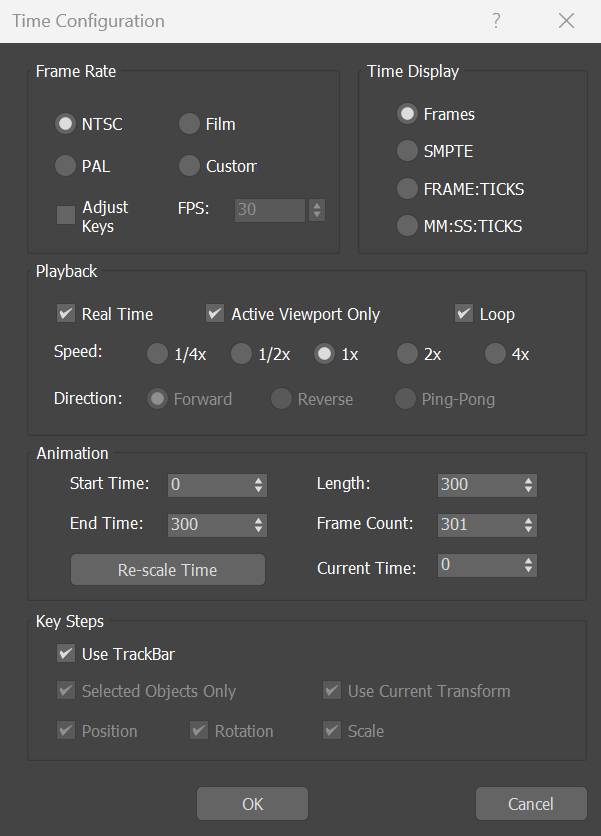
\includegraphics[width=0.5\textwidth]{imagenes/misc/duracion.png}
   \caption{Configuración de la duración de la escena.}
\end{figure}

Como se puede observar, \textit{Frame Count} indica un valor de 301, pero, según la documentación (\href{https://help.autodesk.com/view/3DSMAX/2022/ENU/?guid=GUID-9473CAF3-AF73-4127-A98C-58ACEF01ACAC}{Enlace}), siempre será la longitud más 1, por lo que realmente no hay que fijarse en este valor. Otra forma de comprobar que es correcto es cambiar el \textit{Time Display} a ``MM:SS:TICKS'' y mirando las casillas \textit{End Time} y \textit{Length}, que indican 10 segundos.

\newpage